\section{Mesh processing}\label{mesh}

The mesh processing pipeline is designed to take the generated  \texttt{.stl} files and convert them into a voxelized representation suitable for numerical simulations. This section describes the main steps involved in the mesh processing pipeline as illustrated in Figure \ref{fig:voxelizing}.

\begin{figure}[H]
	\centering
	\vspace{2mm}
	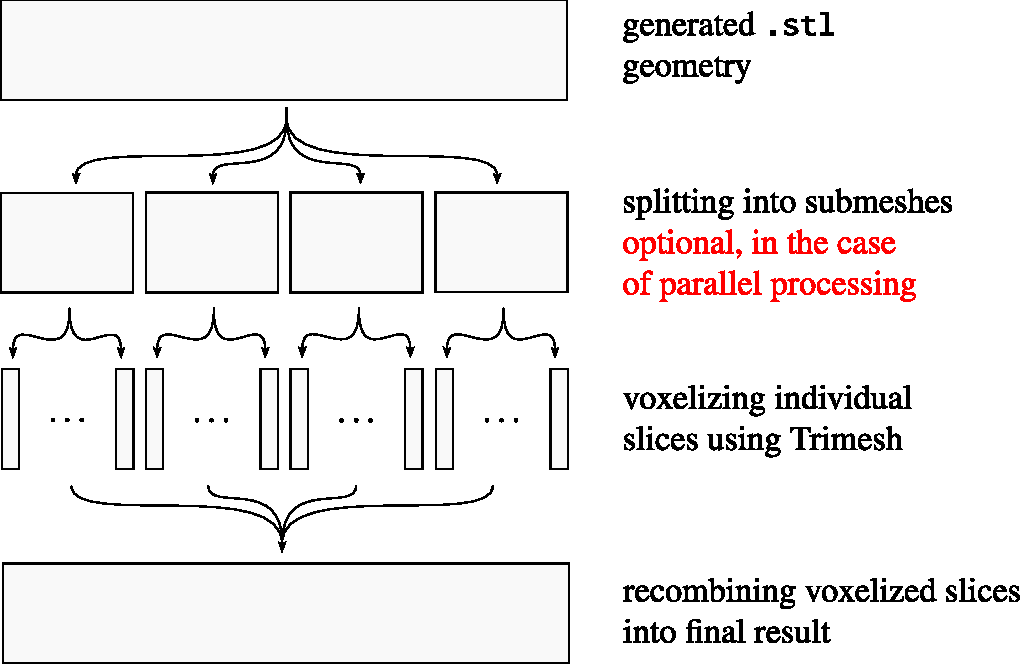
\includegraphics[width=.66\textwidth]{figures/voxelizing.pdf}
	\vspace{2mm}
	\caption{Overview of the mesh processing pipeline, including optional splitting into submeshes, voxelization of slices, and recombination into the final voxelized geometry.}
	\label{fig:voxelizing}
\end{figure}

While the Trimesh package can load and voxelize an \texttt{.stl} file in a single step, this approach becomes computationally expensive for large-scale geometries such as those used in this work. To address this issue, the mesh is split into smaller individual slices along the leading direction, which are then voxelized and recombined. On top of that, the process supports parallelization by grouping the slices into multiple independent groups.

\subsection{Parallel processing of submeshes}\label{parallelization}
 The \texttt{.stl} file can be first loaded as a mesh using the Trimesh package and then divided into smaller submeshes along its leading direction. This division reduces the computational cost by distributing the workload across multiple CPU cores, hence significantly reducing processing time.

The parallelization is achieved by using Python’s \texttt{ProcessPoolExecutor} available in the built-in \texttt{concurrent.futures} module \cite{concurrent-futures}, as shown in Listing \ref{lst:parallel}. The \texttt{ProcessPoolExecutor} allows tasks to be executed in parallel each running independently on separate CPU cores \cite{concurrent-futures}.

\begin{lstlisting}[
language=Python,
caption={Parallel processing of submeshes for voxelization.},
label={lst:parallel}]
# Parallel processing of submeshes
with ProcessPoolExecutor(max_workers=num_processes) as executor:
	# Prepare arguments for each submesh processing
	futures = [
		executor.submit(
		process_submesh,
		submsh,
		margin,
		voxel_size,
		leading_direction
		) for submsh, margin in zip(submeshes, margins)
	]
	
	# Collecting results
	components = [
		future.result() for future in 
		tqdm(futures, total=len(submeshes), desc="Voxelizing")
	]
\end{lstlisting}

\subsection{Voxelization and recombination of slices}\label{voxelizing and recombining}

The mesh, whether processed as a whole or divided into submeshes (if parallelization is used), is split into individual slices based on their thickness that is defined by the user. Each slice is then converted into a voxelized representation using the Trimesh package, which provides a tool for voxelizing 3D geometries, as shown in Listing \ref{lst:voxelize}.

\begin{lstlisting}[
	language=Python,
	caption={Voxelization of a mesh slice using the Trimesh package \cite{trimesh}.},
	label={lst:voxelize}]
def voxelize_elementary(mesh, voxel_size):
	# Voxelize mesh with the specified voxel size
	# In this case, the mesh represents an elementary slice
	return mesh.voxelized(voxel_size).matrix
\end{lstlisting}

Finally, the voxelized slices are recombined using the \texttt{numpy.concatenate} function \cite{numpy} along the leading direction to form the final geometry ready for simulation.


\subsection{The \texttt{Geometry} class: a user-friendly interface}

The \texttt{Geometry} class serves as a high-level interface that encapsulates the entire process of mesh generation. It provides users with control over the voxelization process, including options to define the slice thickness and distribute the workload into parallel tasks. The class also supports visualization and file export in multiple formats.

The \texttt{Geometry} class supports the following key functionalities:
\begin{itemize}
	\item \textbf{Voxelization}: Converts the geometry into a voxelized representation based on a Gmsh \texttt{.geo} template as discussed in \ref{voxelizing and recombining}. 
	
	\item \textbf{Parallel Processing}: Allows users to split the geometry into slices paramater) and process them in parallel across multiple CPU cores as discussed in \ref{parallelization}.
	
	The \texttt{split} parameter determines the number of slices into which the mesh is divided along its leading direction. The \texttt{num\_processes} parameter specifies the number of groups into which the slices are distributed, with each group processed on a separate CPU core. 
	
	\item \textbf{Mesh Exporting}: Exports the voxelized mesh as binary NumPy object (\texttt{.npy}), plain text file (\texttt{.txt}), or LBM simulation-compatible \texttt{.tnl} format. Exporting in the \texttt{.tnl} format is achieved using the PyTNL package \cite{pytnl}, which provides Python bindings for TNL.
	
	\item \textbf{Visualization}: Visualizes the voxelized geometry, primarily for debugging purposes. Visualization is implemented using the Mayavi Python package \cite{mayavi}, which allows inspecting geometries in an interactive 3D environment. An example visualization, generated using the \texttt{.geo} template file from Appendix \ref{appendix B}, is shown in Figure \ref{fig:visualization}.
\end{itemize}

\begin{figure}[H]
	\centering
	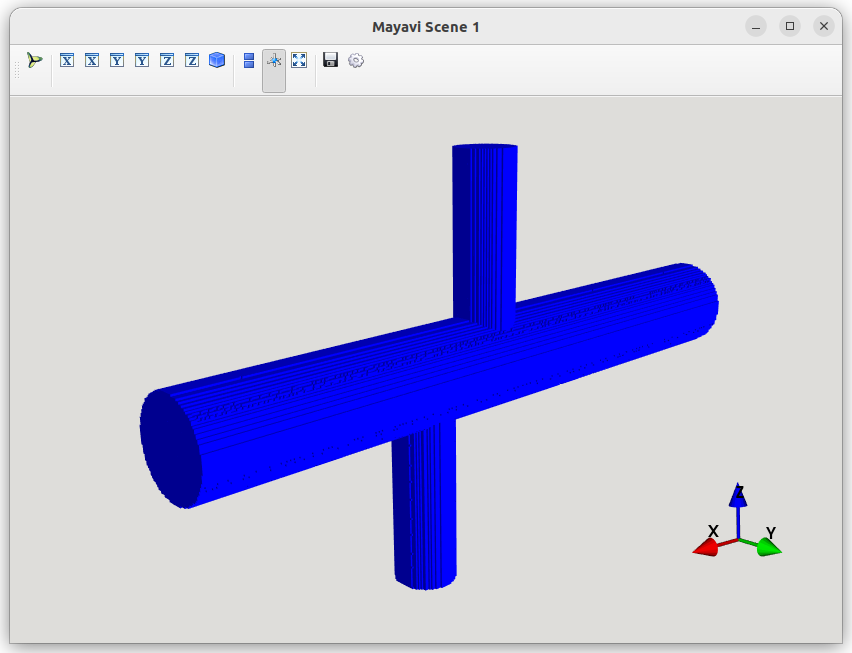
\includegraphics[width=.7\textwidth]{figures/mayavi.png}
	\caption{Visualization of the voxelized geometry using the Mayavi package \cite{mayavi}.}
	\label{fig:visualization}
\end{figure}


Finally, the following code demonstrates the usage of the \texttt{Geometry} class, from defining the object to exporting the voxelized geometry in multiple formats and visualizing it.

\begin{lstlisting}[
	language=Python,
	caption={Example usage of the \texttt{Geometry} class.},
	label={lst:geometry}
	]
from meshgen.geometry import Geometry
	
# Initialize a Geometry instance with parameters
geom = Geometry(
	name="junction_1d",  # name of the .geo template file
	resolution=8,        # desired resolution for the LBM simulation
	split=1024,          # slice thickness; mesh is split into 1024 
						 # slices
	num_processes=8,     # distribute slices into 8 groups, each
						 # processed on a separate CPU core
	offset=0.02,		 # any optimization parameters specific to
						 # the problem
	expected_in_outs={"W", "E", "S", "N"} # list of the parts of the
										  # computational domain that
										  # are expected to include 
										  # the inlets and outlets;
										  # for practical purposes
)
	
# Generate the voxel mesh
geom.generate_voxel_mesh()

# Save the voxel mesh in various formats
geom.save_voxel_mesh("voxel_mesh.npy")
geom.save_voxel_mesh_to_text("voxel_mesh.txt")
geom.save_voxel_mesh_to_tnl("voxel_mesh.tnl")

# Visualize the voxelized geometry
geom.visualize()
\end{lstlisting}
